% This LaTeX document needs to be compiled with XeLaTeX.
\documentclass[10pt]{article}
\usepackage[utf8]{inputenc}
\usepackage{ucharclasses}
\usepackage{graphicx}
\usepackage[export]{adjustbox}
\graphicspath{ {./images/} }
\usepackage{amsmath}
\usepackage{amsfonts}
\usepackage{amssymb}
\usepackage[version=4]{mhchem}
\usepackage{stmaryrd}
\usepackage{hyperref}
\hypersetup{colorlinks=true, linkcolor=blue, filecolor=magenta, urlcolor=cyan,}
\urlstyle{same}
\usepackage{multirow}
\usepackage[fallback]{xeCJK}
\usepackage{polyglossia}
\usepackage{fontspec}
\setCJKmainfont{Noto Serif CJK KR}

\setmainlanguage{polish}
\setotherlanguages{bengali}
\newfontfamily\bengalifont{Noto Serif Bengali}
\newfontfamily\lgcfont{CMU Serif}
\setDefaultTransitions{\lgcfont}{}
\setTransitionsFor{Bengali}{\bengalifont}{\lgcfont}

\title{KOD }

\author{}
\date{}


\newcommand\Varangle{\mathop{{<\!\!\!\!\!\text{\small)}}\:}\nolimits}

\begin{document}
\maketitle
IMIĘ I NAZWISKO *\\
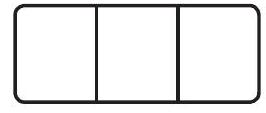
\includegraphics[max width=\textwidth, center]{2024_11_21_1e89351873aa60c4c1b9g-01}\\
\(\square\)

\begin{itemize}
  \item nieobowiązkowe
\end{itemize}

\section*{PRÓBNY EGZAMIN MATURALNY Z NOWĄ ERĄ MATEMATYKA - POZIOM PODSTAWOWY}
\section*{Instrukcja dla zdającego}
\begin{enumerate}
  \item Sprawdź, czy arkusz egzaminacyjny zawiera 22 strony (zadania 1-34) i kartę odpowiedzi. Ewentualny brak stron zgłoś nauczycielowi nadzorującemu egzamin.
  \item Rozwiązania zadań i odpowiedzi zapisz w miejscu na to przeznaczonym.
  \item Pamiętaj, że pominięcie argumentacji lub istotnych obliczeń w rozwiązaniu zadań otwartych może spowodować, że za to rozwiązanie nie otrzymasz pełnej liczby punktów.
  \item Pisz czytelnie. Używaj długopisu/pióra tylko z czarnym tuszem/atramentem.
  \item Nie używaj korektora, a błędne zapisy wyraźnie przekreśl.
  \item Pamiętaj, że zapisy w brudnopisie nie będą oceniane.
  \item Podczas egzaminu możesz korzystać z zestawu wzorów matematycznych, cyrkla i linijki oraz kalkulatora prostego.
  \item Na tej stronie i na karcie odpowiedzi wpisz swój kod oraz imię i nazwisko.
  \item Odpowiedzi do zadań zamkniętych przenieś na kartę odpowiedzi, zaznaczając je w części karty przeznaczonej dla zdającego.
  \item Nie wpisuj żadnych znaków w części przeznaczonej dla osoby sprawdzającej.
\end{enumerate}

Powodzenia!\\
\(\square\) dysleksja

STYCZEŃ 2018

Czas pracy:\\
170 minut

Liczba punktów\\
do uzyskania: 50

W zadaniach od 1. do 25. wybierz i zaznacz na karcie odpowiedzi poprawną odpowiedź.\\
Zadanie 1. (0-1)\\
Liczba \(b\) jest przybliżeniem liczby \(a=\frac{25}{4}\). Błąd względny tego przybliżenia jest równy \(4 \%\). Wskaż błąd bezwzględny tego przybliżenia.\\
A. 0,04\\
B. 0,25\\
C. 0,64\\
D. 2,5

Zadanie 2. (0-1)\\
Liczba odwrotna do \(3-2 \sqrt{2}\) jest równa\\
A. \(3+2 \sqrt{2}\).\\
B. \(2 \sqrt{2}-3\).\\
C. \(3 \sqrt{2}-2\).\\
D. \(2-3 \sqrt{2}\).

Zadanie 3. (0-1)\\
Dla każdej dodatniej liczby \(x\) wyrażenie \(\frac{x \cdot x^{1,5}}{x^{-2}}\) jest równe\\
A. \(x^{-0,75}\).\\
B. \(x^{-0,5}\).\\
C. \(x^{0,5}\).\\
D. \(x^{4,5}\).

\section*{Zadanie 4. (0-1)}
Jeśli \(p=\log _{3} 2\), to liczba \(\log _{3} 36\) jest równa\\
A. \(4 p\).\\
B. \(18 p\).\\
C. \(2 p+2\).\\
D. \(2 p+3\).

Zadanie 5. (0-1)\\
Tabela przedstawia skalę podatkową obowiązującą w 2015 r.

\begin{center}
\begin{tabular}{|c|c|c|}
\hline
\multicolumn{2}{|c|}{Podstawa obliczenia podatku w złotych} & Podatek wynosi \\
\hline
ponad & do &  \\
\hline
 & 85528 & \(18 \%\) minus kwota zmniejszająca podatek \(\mathbf{5 5 6} \mathbf{~ z t ~ 0 2 ~} \mathbf{~ g r}\) \\
\hline
85528 &  & \(14839 \mathrm{zł} 02 \mathrm{gr}+\mathbf{3 2 \%}\) nadwyżki ponad 85528 zt \\
\hline
\end{tabular}
\end{center}

Podstawa obliczenia podatku jest równa \(k\), gdzie \(k<85528\) zł. Wskaż wysokość należnego podatku.\\
A. \((0,18 k-556,02) z ł\)\\
B. \((k-0,18 \cdot 556,02) \mathrm{zł}\)\\
C. \((0,82 k-556,02) \mathrm{zł}\)\\
D. \([14839,02+0,32 \cdot(k-85528)] \mathrm{zł}\)

\section*{Zadanie 6. (0-1)}
Wskaż liczbę spełniającą nierówność: \((2-x)^{2}-9<(x-3)(x+3)\).\\
A. -10\\
B. 0\\
C. 1\\
D. 10

\section*{Zadanie 7. (0-1)}
Równanie \(3 x\left(x^{2}+1\right)\left(x^{3}+8\right)=0\) ma dokładnie\\
A. jedno rozwiązanie rzeczywiste.\\
B. dwa rozwiązania rzeczywiste.\\
C. trzy rozwiązania rzeczywiste.\\
D. cztery rozwiązania rzeczywiste.\\

\includegraphics[max width=\textwidth, center]{2024_11_21_1e89351873aa60c4c1b9g-03}

\section*{Zadanie 8. (0-1)}
Do wykresu funkcji liniowej \(f\) należą punkty \((4,0) \mathrm{i}(0,2)\) oraz punkt\\
A. \((12,-2)\).\\
B. \((12,-4)\).\\
C. \((-12,28)\).\\
D. \((-12,-10)\).

\section*{Zadanie 9. (0-1)}
Na rysunku przedstawiono wykres funkcji \(f\).\\
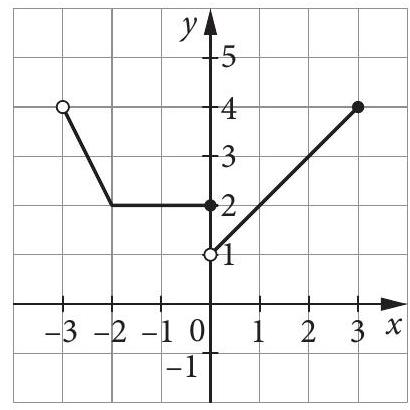
\includegraphics[max width=\textwidth, center]{2024_11_21_1e89351873aa60c4c1b9g-04}

Funkcja \(f\) przyjmuje największą wartość dla \(x\) równego\\
A. -3 .\\
B. 0 .\\
C. 3.\\
D. 4 .

Zadanie 10. (0-1)\\
Liczba -2 jest jednym z miejsc zerowych funkcji kwadratowej \(f(x)=-\frac{1}{2} x^{2}+x+c\). Oblicz \(c\).\\
A. 4\\
B. 2\\
C. 0\\
D. -2

\section*{Zadanie 11. (0-1)}
Wskaż wzór funkcji kwadratowej \(f\), której najmniejsza wartość jest równa 2.\\
A. \(f(x)=-(x-2)^{2}+2\)\\
B. \(f(x)=(x+2)^{2}-2\)\\
C. \(f(x)=2(x-1)^{2}+2\)\\
D. \(f(x)=-2(x-2)^{2}-2\)

\section*{Zadanie 12. (0-1)}
Dane są cztery ciągi określone wzorami ogólnymi dla \(n \geqslant 1\). Który z nich jest ciągiem arytmetycznym?\\
A. \(a_{n}=2 n\)\\
B. \(a_{n}=n^{2}\)\\
C. \(a_{n}=2^{n}\)\\
D. \(a_{n}=\frac{2}{n}\)

Zadanie 13. (0-1)\\
Czwarty wyraz ciągu geometrycznego o wyrazach dodatnich stanowi 0,64 drugiego wyrazu tego ciągu. Wskaż iloraz tego ciągu.\\
A. \(\frac{3}{5}\)\\
B. \(\frac{5}{3}\)\\
C. \(\frac{4}{5}\)\\
D. \(\frac{5}{4}\)

Zadanie 14. (0-1)\\
Wartość \(\cos 120^{\circ}\) jest równa\\
A. \(-\frac{\sqrt{3}}{2}\).\\
B. \(-\frac{1}{2}\).\\
C. \(\frac{1}{2}\).\\
D. \(\frac{\sqrt{3}}{2}\).\\

\includegraphics[max width=\textwidth, center]{2024_11_21_1e89351873aa60c4c1b9g-05}

\section*{Zadanie 15. (0-1)}
Dla pewnego kąta ostrego \(\alpha\) prawdziwa jest równość \(4 \cos \alpha=1\). Miara kąta \(\alpha\) jest\\
A. mniejsza od \(30^{\circ}\).\\
B. równa \(30^{\circ}\).\\
C. równa \(45^{\circ}\).\\
D. większa od \(60^{\circ}\).

\section*{Zadanie 16. (0-1)}
Punkty \(A=(-1,4)\) i \(B=(1,-2)\) są sąsiednimi wierzchołkami rombu \(A B C D\) o polu równym 30 . Sinus kąta ostrego tego rombu jest równy\\
A. \(\frac{3}{4}\).\\
B. \(\frac{\sqrt{7}}{4}\).\\
C. \(\frac{\sqrt{3}}{2}\).\\
D. \(\frac{5}{6}\).

\section*{Zadanie 17. (0-1)}
Punkty \(A, B, C, D\) są położone na okręgu o środku \(S\) tak, jak przedstawiono na rysunku. Odcinek \(A C\) jest średnicą tego okręgu. Wskaż miarę kąta BCA.\\
A. \(18^{\circ}\)\\
B. \(36^{\circ}\)\\
C. \(54^{\circ}\)\\
D. \(72^{\circ}\)\\
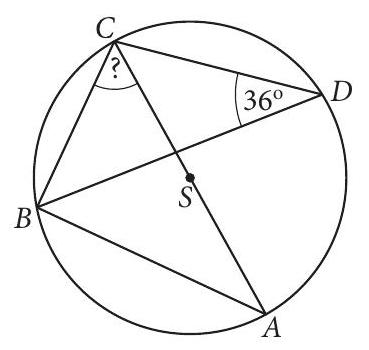
\includegraphics[max width=\textwidth, center]{2024_11_21_1e89351873aa60c4c1b9g-06}

Zadanie 18. (0-1)\\
Z punktu \(P\) poprowadzono dwie styczne do okręgu w punktach \(A\) i \(B\) (zobacz rysunek). Promień okręgu ma długość 5 , a odległość punktu \(P\) od środka \(S\) tego okręgu jest równa 13. Ile wynosi pole deltoidu PBSA?\\
A. 30\\
B. 60\\
C. 64\\
D. 65\\
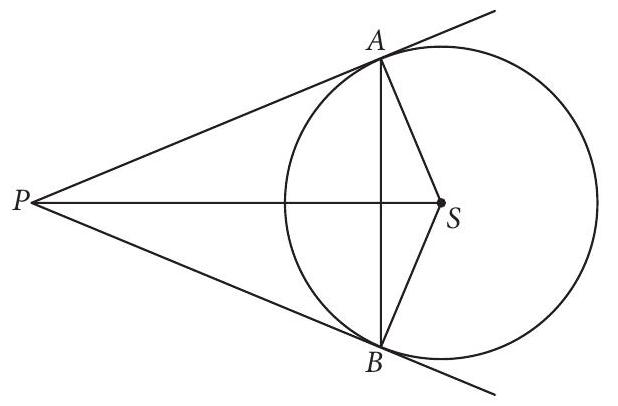
\includegraphics[max width=\textwidth, center]{2024_11_21_1e89351873aa60c4c1b9g-06(1)}

Zadanie 19. (0-1)\\
Jeśli prosta o równaniu \(x+\frac{1}{2} y+a=0\) przechodzi przez punkt \(P=(-1,-2)\), to \(a\) jest równe\\
A. -2 .\\
B. 0 .\\
C. 2 .\\
D. 4 .

Zadanie 20. (0-1)\\
Współczynnik kierunkowy prostej prostopadłej do prostej o równaniu \(2 x+3 y-5=0\) jest równy\\
A. -2 .\\
B. \(-\frac{1}{2}\).\\
C. \(\frac{3}{2}\).\\
D. 2 .

\section*{Zadanie 21. (0-1)}
W walec o przekroju będącym kwadratem wpisano kulę. Jaki jest stosunek pola powierzchni kuli do pola powierzchni całkowitej walca?\\
A. \(\frac{1}{2}\)\\
B. \(\frac{2}{3}\)\\
C. 1\\
D. 2\\

\includegraphics[max width=\textwidth, center]{2024_11_21_1e89351873aa60c4c1b9g-07}

\section*{Zadanie 22. (0-1)}
Krawędź podstawy graniastosłupa prawidłowego czworokątnego jest równa 1. Graniastosłup przecięto płaszczyzną przechodzącą przez krawędź podstawy i tworzącą z tą podstawą kąt \(60^{\circ}\) (zobacz rysunek). Oblicz pole otrzymanego przekroju.\\
A. 1\\
B. \(\frac{2 \sqrt{3}}{3}\)\\
C. \(\sqrt{3}\)\\
D. 2

Zadanie 23. (0-1)\\
Do wazonu w kształcie odwróconego stożka nalano tyle wody, aby sięgnęła do połowy jego wysokości (patrz rysunek). Jaka część objętości wazonu nie została napełniona?\\
A. \(\frac{1}{2}\)\\
B. \(\frac{5}{8}\)\\
C. \(\frac{3}{4}\)\\
D. \(\frac{7}{8}\)\\
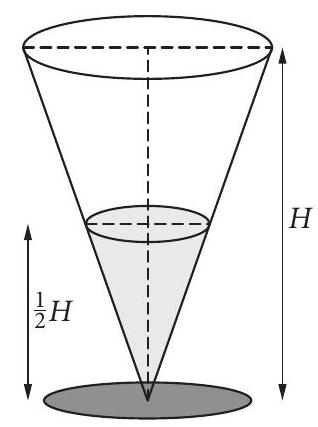
\includegraphics[max width=\textwidth, center]{2024_11_21_1e89351873aa60c4c1b9g-08(1)}

Zadanie 24. (0-1)\\
W pojemniku znajdują się kule białe, czarne i czerwone. Kul białych jest cztery razy więcej niż kul czarnych, a prawdopodobieństwo wylosowania kuli czerwonej jest równe \(\frac{1}{2}\). Losujemy jedną kulę. Ile wynosi prawdopodobieństwo wylosowania kuli białej?\\
A. \(\frac{1}{10}\)\\
B. \(\frac{1}{3}\)\\
C. \(\frac{1}{2}\)\\
D. \(\frac{2}{5}\)

\section*{Zadanie 25. (0-1)}
Na dwa tygodnie przed egzaminem maturalnym uczniom klas trzecich pewnego liceum zadano pytanie: „Ile godzin dziennie poświęcasz nauce?". Wyniki ankiety przedstawiono na diagramie kołowym.

Wskaż średnią liczbę godzin przeznaczonych przez uczniów tej szkoły na naukę.\\
A. 4,5\\
B. 4,9\\
C. 5\\
D. 5,2\\
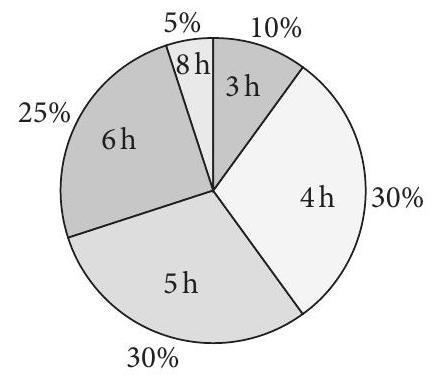
\includegraphics[max width=\textwidth, center]{2024_11_21_1e89351873aa60c4c1b9g-08}\\

\includegraphics[max width=\textwidth, center]{2024_11_21_1e89351873aa60c4c1b9g-09}

Zadanie 26. (0-2)\\
Rozwiąż nierówność: \(x(x-4) \leqslant(2 x+1)(x-4)\).\\

\includegraphics[max width=\textwidth, center]{2024_11_21_1e89351873aa60c4c1b9g-10}

Odpowiedź:

Zadanie 27. (0-2)\\
Ciąg \(\left(a_{n}\right)\) jest określony wzorem \(a_{n}=\frac{4 n+5}{2 n+1}\) dla \(n \geqslant 1\). Sprawdź, czy istnieje wyraz tego ciągu równy \(2 \frac{1}{2}\).

Więcej arkuszy znajdziesz na stronie: \href{http://arkusze.pl}{arkusze.pl}

\begin{center}
\begin{tabular}{|c|c|c|c|c|c|c|c|c|c|c|c|c|c|c|c|c|c|c|c|c|c|c|c|c|c|c|c|c|c|}
\hline
 &  &  &  &  &  &  &  &  &  &  &  &  &  &  &  &  &  &  &  &  &  &  &  &  &  &  &  &  &  \\
\hline
 &  &  &  &  &  &  &  &  &  &  &  &  &  &  &  &  &  &  &  &  &  &  &  &  &  &  &  &  &  \\
\hline
 &  &  &  &  &  &  &  &  &  &  &  &  &  &  &  &  &  &  &  &  &  &  &  &  &  &  &  &  &  \\
\hline
 &  &  &  &  &  &  &  &  &  &  &  &  &  &  &  &  &  &  &  &  &  &  &  &  &  &  &  &  &  \\
\hline
 &  &  &  &  &  &  &  &  &  &  &  &  &  &  &  &  &  &  &  &  &  &  &  &  &  &  &  &  &  \\
\hline
 &  &  &  &  &  &  &  &  &  &  &  &  &  &  &  &  &  &  &  &  &  &  &  &  &  &  &  &  &  \\
\hline
 &  &  &  &  &  &  &  &  &  &  &  &  &  &  &  &  &  &  &  &  &  &  &  &  &  &  &  &  &  \\
\hline
 &  &  &  &  &  &  &  &  &  &  &  &  &  &  &  &  &  &  &  &  &  &  &  &  &  &  &  &  &  \\
\hline
 &  &  &  &  &  &  &  &  &  &  &  &  &  &  &  &  &  &  &  &  &  &  &  &  &  &  &  &  &  \\
\hline
 &  &  &  &  &  &  &  &  &  &  &  &  &  &  &  &  &  &  &  &  &  &  &  &  &  &  &  &  &  \\
\hline
 &  &  &  &  &  &  &  &  &  &  &  &  &  &  &  &  &  &  &  &  &  &  &  &  &  &  &  &  &  \\
\hline
 &  &  &  &  &  &  &  &  &  &  &  &  &  &  &  &  &  &  &  &  &  &  &  &  &  &  &  &  &  \\
\hline
 &  &  &  &  &  &  &  &  &  &  &  &  &  &  &  &  &  &  &  &  &  &  &  &  &  &  &  &  &  \\
\hline
 &  &  &  &  &  &  &  &  &  &  &  &  &  &  &  &  &  &  &  &  &  &  &  &  &  &  &  &  &  \\
\hline
 &  &  &  &  &  &  &  &  &  &  &  &  &  &  &  &  &  &  &  &  &  &  &  &  &  &  &  &  &  \\
\hline
 &  &  &  &  &  &  &  &  &  &  &  &  &  &  &  &  &  &  &  &  &  &  &  &  &  &  &  &  &  \\
\hline
 &  &  &  &  &  &  &  &  &  &  &  &  &  &  &  &  &  &  &  &  &  &  &  &  &  &  &  &  &  \\
\hline
 &  &  &  &  &  &  &  &  &  &  &  &  &  &  &  &  &  &  &  &  &  &  &  &  &  &  &  &  &  \\
\hline
 &  &  &  &  &  &  &  &  &  &  &  &  &  &  &  &  &  &  &  &  &  &  &  &  &  &  &  &  &  \\
\hline
 &  &  &  &  &  &  &  &  &  &  &  &  &  &  &  &  &  &  &  &  &  &  &  &  &  &  &  &  &  \\
\hline
 &  &  &  &  &  &  &  &  &  &  &  &  &  &  &  &  &  &  &  &  &  &  &  &  &  &  &  &  &  \\
\hline
 &  &  &  &  &  &  &  &  &  &  &  &  &  &  &  &  &  &  &  &  &  &  &  &  &  &  &  &  &  \\
\hline
 &  &  &  &  &  &  &  &  &  &  &  &  &  &  &  &  &  &  &  &  &  &  &  &  &  &  &  &  &  \\
\hline
 &  &  &  &  &  &  &  &  &  &  &  &  &  &  &  &  &  &  &  &  &  &  &  &  &  &  &  &  &  \\
\hline
 &  &  &  &  &  &  &  &  &  &  &  &  &  &  &  &  &  &  &  &  &  &  &  &  &  &  &  &  &  \\
\hline
 &  &  &  &  &  &  &  &  &  &  &  &  &  &  &  &  &  &  &  &  &  &  &  &  &  &  &  &  &  \\
\hline
 &  &  &  &  &  &  &  &  &  &  &  &  &  &  &  &  &  &  &  &  &  &  &  &  &  &  &  &  &  \\
\hline
 &  &  &  &  &  &  &  &  &  &  &  &  &  &  &  &  &  &  &  &  &  &  &  &  &  &  &  &  &  \\
\hline
 &  &  &  &  &  &  &  &  &  &  &  &  &  &  &  &  &  &  &  &  &  &  &  &  &  &  &  &  &  \\
\hline
 &  &  &  &  &  &  &  &  &  &  &  &  &  &  &  &  &  &  &  &  &  &  &  &  &  &  &  &  &  \\
\hline
 &  &  &  &  &  &  &  &  &  &  &  &  &  &  &  &  &  &  &  &  &  &  &  &  &  &  &  &  &  \\
\hline
 &  &  &  &  &  &  &  &  &  &  &  &  &  &  &  &  &  &  &  &  &  &  &  &  &  &  &  &  &  \\
\hline
 &  &  &  &  &  &  &  &  &  &  &  &  &  &  &  &  &  &  &  &  &  &  &  &  &  &  &  &  &  \\
\hline
 &  &  &  &  &  &  &  &  &  &  &  &  &  &  &  &  &  &  &  &  &  &  &  &  &  &  &  &  &  \\
\hline
 &  &  &  &  &  &  &  &  &  &  &  &  &  &  &  &  &  &  &  &  &  &  &  &  &  &  &  &  &  \\
\hline
 &  &  &  &  &  &  &  &  &  &  &  &  &  &  &  &  &  &  &  &  &  &  &  &  &  &  &  &  &  \\
\hline
 &  &  &  &  &  &  &  &  &  &  &  &  &  &  &  &  &  &  &  &  &  &  &  &  &  &  &  &  &  \\
\hline
 &  &  &  &  &  &  &  &  &  &  &  &  &  &  &  &  &  &  &  &  &  &  &  &  &  &  &  &  &  \\
\hline
\end{tabular}
\end{center}

Odpowiedź:

\begin{center}
\begin{tabular}{|l|l|c|c|}
\hline
\multirow{2}{*}{\begin{tabular}{c}
Wypełnia \\
sprawdzający \\
\end{tabular}} & Nr zadania & 26 & 27 \\
\cline { 2 - 4 }
 & Maks. liczba pkt & 2 & 2 \\
\cline { 2 - 4 }
 & Uzyskana liczba pkt &  &  \\
\hline
\end{tabular}
\end{center}

Zadanie 28. (0-2)\\
Udowodnij, że nierówność \(\left(x^{2}-3\right)^{2}+x^{4} \geqslant 4 \frac{1}{2}\) jest prawdziwa dla dowolnej liczby rzeczywistej.

Więcej arkuszy znajdziesz na stronie: \href{http://arkusze.pl}{arkusze.pl}\\

\includegraphics[max width=\textwidth, center]{2024_11_21_1e89351873aa60c4c1b9g-12}

\section*{Zadanie 29. (0-2)}
Dla pewnej liczby rzeczywistej \(x\) liczby: \(1-x, 2-3 x, 10+2 x\) są trzema początkowymi wyrazami nieskończonego ciągu arytmetycznego \(\left(a_{n}\right)\), określonego dla \(n \geqslant 1\). Wyznacz \(x\) oraz oblicz sumę dziesięciu początkowych wyrazów tego ciągu.

Więcej arkuszy znajdziesz na stronie: \href{http://arkusze.pl}{arkusze.pl}\\

\includegraphics[max width=\textwidth, center]{2024_11_21_1e89351873aa60c4c1b9g-13}

Odpowiedź:

\begin{center}
\begin{tabular}{|l|l|c|c|}
\hline
\multirow{2}{*}{\begin{tabular}{c}
Wypełnia \\
sprawdzający \\
\end{tabular}} & Nr zadania & 28 & 29 \\
\cline { 2 - 4 }
 & Maks. liczba pkt & 2 & 2 \\
\cline { 2 - 4 }
 & Uzyskana liczba pkt &  &  \\
\hline
\end{tabular}
\end{center}

\section*{Zadanie 30. (0-2)}
Osią symetrii paraboli będącej wykresem funkcji kwadratowej \(f(x)=a x^{2}+b x+3\), gdzie \(a \neq 0\), jest prosta o równaniu \(x=-2\). Wierzchołek paraboli leży na prostej o równaniu \(y=-x+2\). Wyznacz wzór funkcji \(f\) w postaci ogólnej lub kanonicznej.

Więcej arkuszy znajdziesz na stronie: \href{http://arkusze.pl}{arkusze.pl}\\

\includegraphics[max width=\textwidth, center]{2024_11_21_1e89351873aa60c4c1b9g-14}

Odpowiedź:

\section*{Zadanie 31. (0-3)}
Na ściankach symetrycznej dwunastościennej kostki do gry zapisano liczby \(1,2,3, \ldots, 12\) (jak na rysunku). Rzucamy tą kostką trzy razy i zapisujemy wyrzucone liczby w kolejności otrzymywania, tworząc ciąg trójwyrazowy. Oblicz prawdopodobieństwo zdarzenia, że utworzymy w ten sposób ciąg geometryczny o ilorazie całkowitym.\\
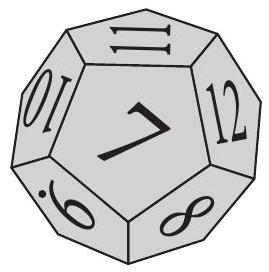
\includegraphics[max width=\textwidth, center]{2024_11_21_1e89351873aa60c4c1b9g-15}

Uwaga. Ciąg stały jest ciągiem geometrycznym.\\

\includegraphics[max width=\textwidth, center]{2024_11_21_1e89351873aa60c4c1b9g-15(1)}

Odpowiedź:

\begin{center}
\begin{tabular}{|l|l|c|c|}
\hline
\multirow{2}{*}{\begin{tabular}{c}
Wypełnia \\
sprawdzający \\
\end{tabular}} & Nr zadania & 30 & 31 \\
\cline { 2 - 4 }
 & Maks. liczba pkt & 2 & 3 \\
\cline { 2 - 4 }
 & Uzyskana liczba pkt &  &  \\
\hline
\end{tabular}
\end{center}

Zadanie 32. (0-3)\\
W ostrosłupie prawidłowym trójkątnym o wysokości \(2 \sqrt{3}\) krawędź boczna tworzy z podstawą kąt \(45^{\circ}\). Oblicz objętość tego ostrosłupa.

Więcej arkuszy znajdziesz na stronie: \href{http://arkusze.pl}{arkusze.pl}\\

\includegraphics[max width=\textwidth, center]{2024_11_21_1e89351873aa60c4c1b9g-16}\\

\includegraphics[max width=\textwidth, center]{2024_11_21_1e89351873aa60c4c1b9g-17}

Odpowiedź:

\begin{center}
\begin{tabular}{|l|l|c|}
\hline
\multirow{2}{*}{\begin{tabular}{c}
Wypełnia \\
sprawdzający \\
\end{tabular}} & Nr zadania & 32 \\
\cline { 2 - 3 }
 & Maks. liczba pkt & 3 \\
\cline { 2 - 3 }
 & Uzyskana liczba pkt &  \\
\hline
\end{tabular}
\end{center}

Zadanie 33. (0-4)\\
W trapezie prostokątnym \(A B C D\) o podstawach \(A B\) i \(C D\) przekątna \(A C\) jest prostopadła do ramienia \(B C\), dłuższa podstawa \(A B\) ma długość 9 , a sinus kąta \(C A D\) jest równy \(\frac{\sqrt{3}}{3}\). Oblicz pole tego trapezu.\\
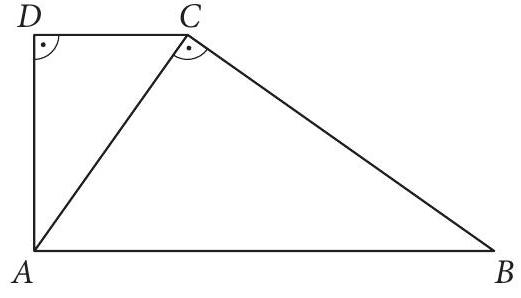
\includegraphics[max width=\textwidth, center]{2024_11_21_1e89351873aa60c4c1b9g-18(1)}

Więcej arkuszy znajdziesz na stronie: \href{http://arkusze.pl}{arkusze.pl}

\begin{center}
\begin{tabular}{|c|c|c|c|c|c|c|c|c|c|c|c|c|c|c|c|c|c|c|c|c|c|c|c|c|c|c|c|c|c|}
\hline
 &  &  &  &  &  &  &  &  &  &  &  &  &  &  &  &  &  &  &  &  &  &  &  &  &  &  &  &  &  \\
\hline
 &  &  &  &  &  &  &  &  &  &  &  &  &  &  &  &  &  &  &  &  &  &  &  &  &  &  &  &  &  \\
\hline
 &  &  &  &  &  &  &  &  &  &  &  &  &  &  &  &  &  &  &  &  &  &  &  &  &  &  &  &  &  \\
\hline
 &  &  &  &  &  &  &  &  &  &  &  &  &  &  &  &  &  &  &  &  &  &  &  &  &  &  &  &  &  \\
\hline
 &  &  &  &  &  &  &  &  &  &  &  &  &  &  &  &  &  &  &  &  &  &  &  &  &  &  &  &  &  \\
\hline
 &  &  &  &  &  &  &  &  &  &  &  &  &  &  &  &  &  &  &  &  &  &  &  &  &  &  &  &  &  \\
\hline
 &  &  &  &  &  &  &  &  &  &  &  &  &  &  &  &  &  &  &  &  &  &  &  &  &  &  &  &  &  \\
\hline
 &  &  &  &  &  &  &  &  &  &  &  &  &  &  &  &  &  &  &  &  &  &  &  &  &  &  &  &  &  \\
\hline
 &  &  &  &  &  &  &  &  &  &  &  &  &  &  &  &  &  &  &  &  &  &  &  &  &  &  &  &  &  \\
\hline
 &  &  &  &  &  &  &  &  &  &  &  &  &  &  &  &  &  &  &  &  &  &  &  &  &  &  &  &  &  \\
\hline
 &  &  &  &  &  &  &  &  &  &  &  &  &  &  &  &  &  &  &  &  &  &  &  &  &  &  &  &  &  \\
\hline
 &  &  &  &  &  &  &  &  &  &  &  &  &  &  &  &  &  &  &  &  &  &  &  &  &  &  &  &  &  \\
\hline
 &  &  &  &  &  &  &  &  &  &  &  &  &  &  &  &  &  &  &  &  &  &  &  &  &  &  &  &  &  \\
\hline
 &  &  &  &  &  &  &  &  &  &  &  &  &  &  &  &  &  &  &  &  &  &  &  &  &  &  &  &  &  \\
\hline
 &  &  &  &  &  &  &  &  &  &  &  &  &  &  &  &  &  &  &  &  &  &  &  &  &  &  &  &  &  \\
\hline
 &  &  &  &  &  &  &  &  &  &  &  &  &  &  &  &  &  &  &  &  &  &  &  &  &  &  &  &  &  \\
\hline
 &  &  &  &  &  &  &  &  &  &  &  &  &  &  &  &  &  &  &  &  &  &  &  &  &  &  &  &  &  \\
\hline
 &  &  &  &  &  &  &  &  &  &  &  &  &  &  &  &  &  &  &  &  &  &  &  &  &  &  &  &  &  \\
\hline
 &  &  &  &  &  &  &  &  &  &  &  &  &  &  &  &  &  &  &  &  &  &  &  &  &  &  &  &  &  \\
\hline
 &  &  &  &  &  &  &  &  &  &  &  &  &  &  &  &  &  &  &  &  &  &  &  &  &  &  &  &  &  \\
\hline
 &  &  &  &  &  &  &  &  &  &  &  &  &  &  &  &  &  &  &  &  &  &  &  &  &  &  &  &  &  \\
\hline
 &  &  &  &  &  &  &  &  &  &  &  &  &  &  &  &  &  &  &  &  &  &  &  &  &  &  &  &  &  \\
\hline
 &  &  &  &  &  &  &  &  &  &  &  &  &  & 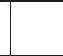
\includegraphics[max width=\textwidth]{2024_11_21_1e89351873aa60c4c1b9g-18}
 &  &  &  &  &  &  &  &  &  &  &  &  &  &  &  \\
\hline
 &  &  &  &  &  &  &  &  &  &  &  &  &  &  &  &  &  &  &  &  &  &  &  &  &  &  &  &  &  \\
\hline
 &  &  &  &  &  &  &  &  &  &  &  &  &  &  &  &  &  &  &  &  &  &  &  &  &  &  &  &  &  \\
\hline
 & 
\includegraphics[max width=\textwidth]{2024_11_21_1e89351873aa60c4c1b9g-18(2)}
 &  &  &  &  &  &  &  &  &  &  &  &  &  &  &  &  &  &  &  &  &  &  &  &  &  &  &  &  \\
\hline
 &  &  &  &  &  &  &  &  &  &  &  &  &  &  &  &  &  &  &  &  &  &  &  &  &  &  &  &  &  \\
\hline
 &  &  &  &  &  &  &  &  &  &  &  &  &  &  &  &  &  &  &  &  &  &  &  &  &  &  &  &  &  \\
\hline
 &  &  &  &  &  &  &  &  &  &  &  &  &  &  &  &  &  &  &  &  &  &  &  &  &  &  &  &  &  \\
\hline
 &  &  &  &  &  &  &  &  &  &  &  &  &  & \textbackslash  &  &  &  &  &  & \textbackslash  &  &  &  &  &  &  &  &  &  \\
\hline
 &  &  &  &  &  &  &  &  &  &  &  &  & - & - &  &  &  &  &  &  &  &  &  &  &  &  &  &  &  \\
\hline
 &  &  &  &  &  &  &  &  &  &  &  &  &  &  &  &  &  &  &  &  &  &  &  &  &  &  &  &  &  \\
\hline
 &  &  &  &  &  &  &  &  &  &  &  &  &  &  &  &  &  &  &  &  &  &  &  &  &  &  &  &  &  \\
\hline
 &  &  &  &  &  &  &  &  &  &  &  &  &  &  &  &  &  &  &  &  &  &  &  &  &  &  &  &  &  \\
\hline
 &  &  &  &  &  &  &  &  &  &  &  &  &  &  &  &  &  &  &  &  &  &  &  &  &  &  &  &  &  \\
\hline
 &  &  &  &  &  &  &  &  &  &  &  &  &  &  &  &  &  &  &  &  &  &  &  &  &  &  &  &  &  \\
\hline
 &  &  &  &  &  &  &  &  &  &  &  &  &  &  &  &  &  &  &  &  &  &  &  &  &  &  &  &  &  \\
\hline
\end{tabular}
\end{center}

\begin{center}

\includegraphics[max width=\textwidth]{2024_11_21_1e89351873aa60c4c1b9g-19}
\end{center}

Odpowiedź:

\begin{center}
\begin{tabular}{|l|l|c|}
\hline
\multirow{2}{*}{\begin{tabular}{c}
Wypełnia \\
sprawdzający \\
\end{tabular}} & Nr zadania & 33 \\
\cline { 2 - 3 }
 & Maks. liczba pkt & 4 \\
\cline { 2 - 3 }
 & Uzyskana liczba pkt &  \\
\hline
\end{tabular}
\end{center}

Zadanie 34. (0-5)\\
W trójkącie \(A B C\) wierzchołek \(A\) ma współrzędne ( 1,6 ), wierzchołek \(B\) leży na osi \(O y, a|\Varangle A C B|=90^{\circ}\).\\
Prosta o równaniu \(y=\frac{1}{2} x+\frac{1}{2}\) jest równoległa do boku \(B C\) i przecina każdy z boków \(A B\) i \(A C\) w połowie. Wyznacz współrzędne wierzchołków \(B\) i \(C\) tego trójkąta.

Więcej arkuszy znajdziesz na stronie: \href{http://arkusze.pl}{arkusze.pl}\\

\includegraphics[max width=\textwidth, center]{2024_11_21_1e89351873aa60c4c1b9g-20}\\

\includegraphics[max width=\textwidth, center]{2024_11_21_1e89351873aa60c4c1b9g-21}

Odpowiedź:

\begin{center}
\begin{tabular}{|l|l|c|}
\hline
\multirow{2}{*}{\begin{tabular}{c}
Wypełnia \\
sprawdzający \\
\end{tabular}} & Nr zadania & 34 \\
\cline { 2 - 3 }
 & Maks. liczba pkt & 5 \\
\cline { 2 - 3 }
 & Uzyskana liczba pkt &  \\
\hline
\end{tabular}
\end{center}

\begin{center}

\includegraphics[max width=\textwidth]{2024_11_21_1e89351873aa60c4c1b9g-22}
\end{center}

\section*{WPISUJE ZDAJĄCY}
\begin{center}
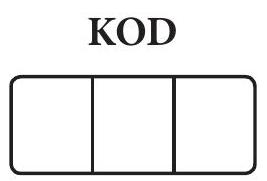
\includegraphics[max width=\textwidth]{2024_11_21_1e89351873aa60c4c1b9g-23(1)}
\end{center}

IMIĘ I NAZWISKO *

\begin{itemize}
  \item nieobowiązkowe
\end{itemize}

KARTA ODPOWIEDZI

\begin{center}
\begin{tabular}{|c|c|c|c|c|c|}
\hline
 & \( \mathrm{Nr} \) &  & Odp & viedzi &  \\
\hline
 & 1 & A & B & C & D \\
\hline
 & 2 & A & B & C & D \\
\hline
 & 3 & A & B & C & D \\
\hline
 & 4 & A & B & C & D \\
\hline

\includegraphics[max width=\textwidth]{2024_11_21_1e89351873aa60c4c1b9g-23(2)}
 & 5 & A & B & C & D \\
\hline
N & 6 & A & B & C & D \\
\hline
돔 & 7 & A & B & C & C \\
\hline
\( \ddot{~} \) & 8 & A & B & C & D \\
\hline
응 & 9 & A & B & C & D \\
\hline
g & 10 & A & B & C & D \\
\hline

\includegraphics[max width=\textwidth]{2024_11_21_1e89351873aa60c4c1b9g-23}
 & 11 & A & B & C & D \\
\hline
\( \frac{N}{D} \) & 12 & A & B & C & D \\
\hline
\( \tilde{\tilde{N}} \) & 13 & A & B & C & D \\
\hline
స్ & 14 & A & B & C & D \\
\hline
菅 & 15 & A & B & C & D \\
\hline
'ষ্ট & 16 & A & B & C & D \\
\hline
 & 17 & A & B & C & D \\
\hline
 & 18 & A & B & C & D \\
\hline
 & 19 & A & B & C & D \\
\hline
 & 20 & A & B & C & D \\
\hline
 & 21 & A & B & C & D \\
\hline
 & 22 & A & B & C & D \\
\hline
 & 23 & A & B & C & D \\
\hline
 & 24 & A & B & C & D \\
\hline
 & 25 & A & B & C & D \\
\hline
\end{tabular}
\end{center}

WYPEENIA SPRAWDZAJĄCY

\begin{center}
\begin{tabular}{|c|c|c|c|c|c|c|}
\hline
\multirow{2}{*}{\begin{tabular}{c}
Nr \\
zad. \\
\end{tabular}} & \multicolumn{6}{|c|}{Punkty} \\
\hline
 & \(\mathbf{0}\) & \(\mathbf{1}\) & \(\mathbf{2}\) & \(\mathbf{3}\) & \(\mathbf{4}\) & \(\mathbf{5}\) \\
\hline
\(\mathbf{2 6}\) & \(\square\) & \(\square\) & \(\square\) &  &  &  \\
\hline
\(\mathbf{2 7}\) & \(\square\) & \(\square\) & \(\square\) &  &  &  \\
\hline
\(\mathbf{2 8}\) & \(\square\) & \(\square\) & \(\square\) &  &  &  \\
\hline
\(\mathbf{2 9}\) & \(\square\) & \(\square\) & \(\square\) &  &  &  \\
\hline
\(\mathbf{3 0}\) & \(\square\) & \(\square\) & \(\square\) &  &  &  \\
\hline
\(\mathbf{3 1}\) & \(\square\) & \(\square\) & \(\square\) & \(\square\) &  &  \\
\hline
\(\mathbf{3 2}\) & \(\square\) & \(\square\) & \(\square\) & \(\square\) &  &  \\
\hline
\(\mathbf{3 3}\) & \(\square\) & \(\square\) & \(\square\) & \(\square\) & \(\square\) &  \\
\hline
\(\mathbf{3 4}\) & \(\square\) & \(\square\) & \(\square\) & \(\square\) & \(\square\) & \(\square\) \\
\hline
\end{tabular}
\end{center}


\end{document}